\documentclass[conference]{IEEEtran}
\IEEEoverridecommandlockouts
% Times/Courier clones when compiled with XeTeX (e.g. Tectonic); pdfLaTeX/Overleaf skip this
\usepackage{iftex}
\ifXeTeX
  \usepackage{fontspec}
  \setmainfont{texgyretermes}[Extension=.otf, UprightFont=*-regular,
    BoldFont=*-bold, ItalicFont=*-italic, BoldItalicFont=*-bolditalic]
  \setmonofont{texgyrecursor}[Extension=.otf, UprightFont=*-regular,
    BoldFont=*-bold, ItalicFont=*-italic, BoldItalicFont=*-bolditalic]
\fi
\usepackage{cite}
\usepackage{amsmath,amssymb,amsfonts}
\usepackage{graphicx}
\usepackage{textcomp}
\usepackage{xcolor}
\usepackage{booktabs}
\usepackage{tikz}
\usetikzlibrary{positioning,arrows.meta}
\usepackage{url}

\begin{document}

\title{Griev.AI.ance: Routing Consumer Financial Complaints with Machine Learning\\
{\large CSC 4850 Final Project Report}}

\author{
\IEEEauthorblockN{Raina Bethea}
\IEEEauthorblockA{\textit{Dept. of Computer Science}\\
\textit{Georgia State University}\\
Atlanta, GA, USA}
\and
\IEEEauthorblockN{Omar Elkady}
\IEEEauthorblockA{\textit{Dept. of Computer Science}\\
\textit{Georgia State University}\\
Atlanta, GA, USA}
\and
\IEEEauthorblockN{Victor Googe}
\IEEEauthorblockA{\textit{Dept. of Computer Science}\\
\textit{Georgia State University}\\
Atlanta, GA, USA}
}

\maketitle

\begin{abstract}
Every complaint sent to the U.S.\ Consumer Financial Protection Bureau (CFPB) has to reach the team that handles its financial product, and complaints that will end in monetary relief deserve early attention. Griev.AI.ance reads the free-text narrative of a complaint and (1)~predicts its product among 11 categories and (2)~scores how likely it is to close with monetary relief. We built a 162,500-complaint dataset from 1.18 million unique narratives filed between August 2023 and July 2026, rebuilt from an archived copy of the CFPB database after the bureau stopped publishing narratives. We compared eight classifiers under one protocol (a fixed 80/20 split and 3-fold cross-validated tuning). A linear SVM on word and bigram TF-IDF features reached 0.784 macro-F1 and 80.6\% accuracy, up from 0.695 for our naive Bayes baseline, and beat every nonlinear model trained on truncated-SVD features. For monetary relief (5.6\% positive), logistic regression on text, product and company reached a PR-AUC of 0.393, seven times the base rate. We also show how much truncated SVD loses, what k-means finds in the narratives, which words drive the predictions, and where the model fails.
\end{abstract}

\begin{IEEEkeywords}
text classification, consumer complaints, CFPB, TF-IDF, linear SVM, truncated SVD, imbalanced classification
\end{IEEEkeywords}

\section{Introduction}
The CFPB forwards complaints about credit reports, debt collectors, bank accounts, loans and other financial products to the companies involved and publishes them in its Consumer Complaint Database~\cite{cfpb}. The volume is large: more than 2.3 million complaints with a narrative were filed between August 2023 and July 2026. Each complaint has to get to the team that handles its product, and the small share that ends in monetary relief is the most costly for companies and the most important for consumers. A model that reads the narrative could route new complaints automatically, flag complaints whose label does not match the text, and help with triage.

We treat routing as supervised multi-class text classification: the input is the consumer's narrative and the target is one of the 11 CFPB product categories. Because some products have far more complaints than others, macro-F1 is our main metric. Our secondary task is binary: will the complaint close with monetary relief? This report covers the full project. Our contributions are:
\begin{itemize}
\item a reproducible dataset rebuilt from the last public copy of the CFPB narratives, with template letters and ambiguous labels removed;
\item a comparison of eight classifiers for product routing under one split and one tuning protocol;
\item a monetary-relief model evaluated with imbalance-aware metrics against a prevalence baseline;
\item an analysis of truncated SVD and k-means clustering, explanations of the predictions, an error analysis and a leakage check; and
\item a Streamlit demo that routes a pasted complaint and explains its prediction.
\end{itemize}

\section{Related Work}
\textit{Classical text classification.} Joachims~\cite{joachims} showed that linear SVMs suit text, which has many sparse but relevant features, and that they beat naive Bayes, Rocchio, $k$-NN and C4.5 on the Reuters and Ohsumed benchmarks. McCallum and Nigam~\cite{mccallum} found that the multinomial event model of naive Bayes beats the Bernoulli model with large vocabularies, and Rennie et al.~\cite{rennie} fixed several of its weak assumptions, for example with Complement NB for skewed classes. Latent semantic analysis~\cite{lsa} applies a truncated SVD to the term--document matrix to get dense, low-rank text features. These papers shaped our plan: start with naive Bayes, move to linear models, and test whether truncated SVD keeps enough information for nonlinear models.

\textit{CFPB complaints.} Bastani et al.~\cite{bastani} used LDA topic models on CFPB narratives to surface consumer issues automatically. Pradhan et al.~\cite{pradhan} classified CFPB complaints with large language models and found that few-shot prompts built from the most similar labeled complaints beat zero-shot prompting and also beat fine-tuned RoBERTa, SVM and logistic regression baselines. Wang et al.~\cite{wang} predicted monetary relief with XGBoost on narrative text, topics and company and state fields, evaluated on a temporal split, and raised ROC-AUC from 0.69 for a TF-IDF baseline to 0.78. Our work differs in that product routing is the main task, all classical models share one split and one tuning protocol, and we study what dimensionality reduction costs.

\section{Dataset}
\label{sec:data}
\textit{Source.} We use the CFPB Consumer Complaint Database~\cite{cfpb}. Each complaint has 16 fields, including the product, sub-product, issue, company, the company's response and the narrative. Narratives are published only with the consumer's consent, after personal details are replaced with placeholders such as \texttt{XXXX}. On August 14, 2026 the CFPB stopped publishing narratives: the current bulk file and API no longer contain them. Our first exports were made before that date, but to make the project reproducible we rebuilt the data from the full bulk file as archived by the Internet Archive on August 15, 2026 (1.4~GB compressed, 17.1 million complaints). We keep complaints received from August 1, 2023, when the CFPB last revised its product categories, so all labels use the same 11 products. The latest narrative in the archive is from July 27, 2026.

\textit{Cleaning.} Table~\ref{tab:funnel} shows each step. Text cleaning lowercases the narrative, replaces dollar amounts such as \texttt{\{\$200.00\}} with one token, \texttt{dollaramount}, removes redacted names and dates, and collapses whitespace. The biggest data-quality problem is template letters. Almost half of the narratives repeat another one after cleaning, and the largest group of identical narratives has 29,024 copies (a credit-report dispute letter). We keep the earliest copy of each narrative. A narrative filed under more than one product has no single correct label, so we drop every copy of the 1,924 such texts (282,505 complaints). This leaves 1,183,581 unique, unambiguous narratives.

\begin{table}[!t]
\caption{Data Cleaning Funnel}
\label{tab:funnel}
\centering
\footnotesize
\begin{tabular}{@{}lr@{}}
\toprule
Stage & Complaints \\
\midrule
Rows in the archived CFPB file (all years) & 17,119,590 \\
Narratives received Aug 2023--Jul 2026 & 2,355,520 \\
\quad dropped: under three words after cleaning & 1,191 \\
\quad dropped: pre-2023 product names & 29,818 \\
\quad dropped: duplicate narratives & 1,139,006 \\
\quad dropped: same text under several products & 282,505 \\
Unique, unambiguous narratives & 1,183,581 \\
Modeling sample (130,000 train / 32,500 test) & 162,500 \\
\bottomrule
\end{tabular}
\end{table}

\textit{Sampling and split.} Credit reporting makes up 53.3\% of the unique narratives and debt or credit management only 0.45\%. We drew a random sample capped per product, from 35,000 complaints for credit reporting down to 5,000 for prepaid cards and debt or credit management, for a total of 162,500. This lowers the ratio between the largest and smallest class from 119:1 to 7:1. We split the sample once, 80/20 and stratified by product (seed 42), and stored the split in the data so that every model trains and tests on the same complaints. Because of the caps, our test metrics describe a more balanced mix of products than the CFPB actually receives.

\textit{Exploration.} Narrative lengths are right-skewed: the median is 156 words, the mean 219 and the longest 5,939. Mortgage narratives are the longest (median 220 words) and debt or credit management and money transfer the shortest (110). Some products have very distinctive words, often company names (\textit{mohela} and \textit{nelnet} for student loans, \textit{zelle} and \textit{cash app} for money transfer, \textit{escrow} for mortgages), while others share generic words such as \textit{credit}, \textit{account} and \textit{payment}.

\textit{Monetary relief label.} A complaint is positive if the company's response is ``Closed with monetary relief.'' The 1,907 complaints that were still in progress or got an untimely response have no final outcome and are left out of this task. Of the remaining 160,593 complaints, 5.7\% are positive (5.6\% in the test set).

\begin{figure*}[!t]
\centering
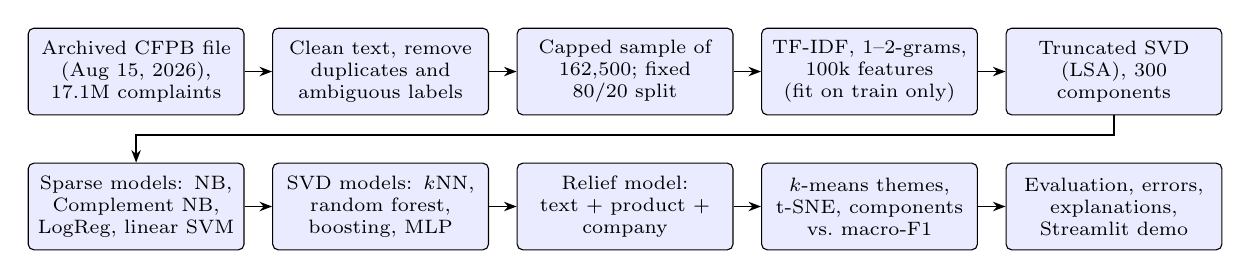
\begin{tikzpicture}[
  node distance=3mm and 3.5mm,
  stage/.style={draw, rounded corners=2pt, align=center, font=\scriptsize,
                text width=26mm, minimum height=11mm, inner sep=2pt, fill=blue!8},
  arr/.style={-{Stealth[length=1.6mm]}, semithick}]
\node[stage] (data) {Archived CFPB file\\(Aug 15, 2026),\\17.1M complaints};
\node[stage, right=of data] (clean) {Clean text, remove\\duplicates and\\ambiguous labels};
\node[stage, right=of clean] (sample) {Capped sample of\\162,500; fixed\\80/20 split};
\node[stage, right=of sample] (tfidf) {TF-IDF, 1--2-grams,\\100k features\\(fit on train only)};
\node[stage, right=of tfidf] (svd) {Truncated SVD\\(LSA), 300\\components};
\node[stage, below=6mm of data] (sparse) {Sparse models: NB,\\Complement NB,\\LogReg, linear SVM};
\node[stage, right=of sparse] (dense) {SVD models: $k$NN,\\random forest,\\boosting, MLP};
\node[stage, right=of dense] (relief) {Relief model:\\text + product +\\company};
\node[stage, right=of relief] (clus) {$k$-means themes,\\t-SNE, components\\vs.\ macro-F1};
\node[stage, right=of clus] (eval) {Evaluation, errors,\\explanations,\\Streamlit demo};
\foreach \a/\b in {data/clean, clean/sample, sample/tfidf, tfidf/svd,
                   sparse/dense, dense/relief, relief/clus, clus/eval}
  \draw[arr] (\a) -- (\b);
\draw[arr] (svd.south) -- ++(0,-2.5mm) -| (sparse.north);
\end{tikzpicture}
\caption{Project pipeline. Every model reads the same processed dataset and the same train/test split; all tuning happens inside the training set.}
\label{fig:pipeline}
\end{figure*}

\section{Methods}
Fig.~\ref{fig:pipeline} shows the pipeline.

\textit{Features.} Each narrative becomes a TF-IDF vector $\mathbf{x}\in\mathbb{R}^{|V|}$ over unigrams and bigrams, with English stop words removed. A term is kept if it appears in at least 5 and at most 90\% of training documents, and the 100,000 most frequent terms form the vocabulary. Term frequencies are sublinear, $1+\log \mathrm{tf}$, and every vector is L2-normalized. The vectorizer is fitted on the training set only.

\textit{Sparse classifiers.} Multinomial naive Bayes (MNB) predicts
\begin{equation}
\hat{c} = \arg\max_{c}\Big[\log \pi_c + \sum_{j} x_j \log \theta_{cj}\Big],\quad
\theta_{cj} = \frac{N_{cj}+\alpha}{N_c+\alpha|V|},
\end{equation}
where $\pi_c$ is the class prior, $N_{cj}$ the total weight of term $j$ in class $c$, and $\alpha$ the smoothing constant. Complement NB~\cite{rennie} estimates $\theta$ from all classes except $c$, which helps small classes. Multinomial logistic regression models $P(c\mid\mathbf{x}) \propto \exp(\mathbf{w}_c^\top\mathbf{x}+b_c)$ and minimizes the cross-entropy plus an L2 penalty with weight $1/C$. The linear SVM trains one classifier per product (one vs.\ rest) by minimizing
\begin{equation}
\tfrac{1}{2}\lVert\mathbf{w}\rVert^2 + C\sum_i s_i \max\!\big(0,\,1-y_i\mathbf{w}^\top\mathbf{x}_i\big)^2,
\end{equation}
where $s_i$ is an optional class weight inversely proportional to class size.

\textit{Dense classifiers.} Neighbor search, trees and neural networks scale poorly to 100,000 sparse dimensions, so $k$-NN, random forest, histogram gradient boosting and a multilayer perceptron (MLP) use a truncated SVD of the TF-IDF matrix, $\mathbf{X}\approx\mathbf{U}_k\boldsymbol{\Sigma}_k\mathbf{V}_k^\top$, with features $\mathbf{z}=\mathbf{V}_k^\top\mathbf{x}$ and $k=300$. For $k$-NN the vectors are L2-normalized, so Euclidean distance ranks neighbors the same way as cosine similarity. The MLP has one ReLU hidden layer and is trained with Adam and early stopping on a 10\% validation split.

\textit{Tuning protocol.} Every model is tuned with 3-fold stratified cross-validation on the training set, using macro-F1. The grids cover $\alpha$ for naive Bayes; $C$ and balanced vs.\ no class weights for the linear models; $k$ and the vote weights for $k$-NN; tree depth and leaf size for the random forest; learning rate and leaf count for boosting; and hidden size and L2 penalty for the MLP. For the four slower SVD models, the grid search runs on a stratified 30,000-complaint subsample. The best setting is then refitted on all 130,000 training complaints and scored once on the test set.

\textit{Monetary relief.} We compare a prevalence baseline with class-weighted logistic regression on five feature sets: product only; text only; text + product; text + product + company (the 50 most common companies plus ``Other,'' one-hot encoded); and a linear SVM on the last set. The positive class is weighted inversely to its frequency. Because positives are rare, we score with ROC-AUC and PR-AUC (average precision). The decision threshold is the one that maximizes F1 on out-of-fold training predictions, so the test set is never used for a choice.

\textit{Unsupervised analysis.} We measure macro-F1 for a linear SVM trained on the first $k$ SVD components ($k$ from 2 to 500), plot the complaints in 2-D with SVD and t-SNE~\cite{tsne}, and run k-means on L2-normalized 100-component LSA vectors. We pick $k$ by silhouette score and compare the clusters with the product labels using the adjusted Rand index (ARI) and normalized mutual information (NMI).

\textit{Metrics.} For routing we report accuracy, per-class precision, recall and F1, and macro-F1, $\frac{1}{K}\sum_{c} F1_c$, which weights all 11 products equally. All experiments use scikit-learn~\cite{sklearn} with \texttt{random\_state=42}, and a full rerun reproduces every number in this report.

\section{Experiments and Results}

\subsection{Product Routing}
Table~\ref{tab:results} compares all models. The linear SVM is best, with test macro-F1 0.784 and accuracy 80.6\%, and logistic regression is close behind (0.776). Cross-validation and test scores agree closely (0.777 vs.\ 0.784 for the SVM), so the tuning did not overfit. Compared with our mid-term baseline (naive Bayes on 5,000 unigrams, scored on the same test set), the SVM gains 0.089 macro-F1. Of that gain, 0.028 comes from better features and tuning alone: MNB with bigrams, a 100,000-term vocabulary and $\alpha=0.03$ reaches 0.723. The rest comes from the discriminative models.

\begin{table}[!t]
\caption{Product Routing on the 32,500-Complaint Test Set}
\label{tab:results}
\centering
\footnotesize
\setlength{\tabcolsep}{3.5pt}
\begin{tabular}{@{}llccr@{}}
\toprule
Model & Features & Macro-F1 & Acc. & Train (s) \\
\midrule
NB, mid-term baseline & 5k unigrams & 0.695 & 0.728 & -- \\
\midrule
Multinomial NB & TF-IDF 100k & 0.723 & 0.749 & 0.5 \\
Complement NB & TF-IDF 100k & 0.721 & 0.759 & 0.5 \\
Logistic regression & TF-IDF 100k & 0.776 & 0.798 & 94 \\
\textbf{Linear SVM} & TF-IDF 100k & \textbf{0.784} & \textbf{0.806} & 66 \\
\midrule
$k$-NN ($k=35$) & SVD-300 & 0.709 & 0.751 & 0.2 \\
Random forest & SVD-300 & 0.707 & 0.749 & 354 \\
Gradient boosting & SVD-300 & 0.734 & 0.765 & 186 \\
MLP (256 units) & SVD-300 & 0.747 & 0.777 & 29 \\
\bottomrule
\end{tabular}
\end{table}

\textit{Sparse linear models win.} All four models trained on SVD-300 features score below logistic regression and the SVM on the full TF-IDF matrix. The best of them, the MLP, reaches 0.747. Section~\ref{sec:svd} shows why: compressing to 300 components already costs a linear model about 0.05 macro-F1, and the nonlinear models do not win it back. This matches Joachims's argument that text has many relevant sparse features~\cite{joachims}. The linear models are also practical: they train in one to two minutes and predict almost instantly, while $k$-NN needs 22~s just to predict the test set and the random forest takes six minutes to train.

\textit{Per-product results.} Table~\ref{tab:perclass} shows F1 per product. Student loans (0.918) and mortgages (0.916) are easiest because their vocabulary and servicer names are distinctive. The hardest product is debt or credit management (0.501), whose complaints read like debt-collection or credit-report complaints, followed by payday and personal loans (0.691). The SVM improves every product over naive Bayes, most of all money transfer (+0.111), credit cards and payday loans (+0.088 each).

\begin{table}[!t]
\caption{Test F1 per Product for Four Models}
\label{tab:perclass}
\centering
\footnotesize
\setlength{\tabcolsep}{4pt}
\begin{tabular}{@{}lcccc@{}}
\toprule
Product (test size) & MNB & MLP & LogReg & SVM \\
\midrule
Checking/savings (4,000) & 0.721 & 0.753 & 0.776 & 0.788 \\
Credit card (4,000) & 0.715 & 0.762 & 0.791 & 0.803 \\
Credit reporting (7,000) & 0.808 & 0.829 & 0.831 & 0.839 \\
Debt collection (5,000) & 0.729 & 0.752 & 0.766 & 0.776 \\
Debt/credit mgmt.\ (1,000) & 0.457 & 0.453 & 0.500 & 0.501 \\
Money transfer (3,000) & 0.690 & 0.775 & 0.790 & 0.801 \\
Mortgage (2,000) & 0.878 & 0.889 & 0.914 & 0.916 \\
Payday/personal loan (1,500) & 0.603 & 0.604 & 0.673 & 0.691 \\
Prepaid card (1,000) & 0.685 & 0.706 & 0.762 & 0.752 \\
Student loan (2,000) & 0.897 & 0.895 & 0.908 & 0.918 \\
Vehicle loan/lease (2,000) & 0.769 & 0.798 & 0.824 & 0.835 \\
\bottomrule
\end{tabular}
\end{table}

\textit{Confusions.} The SVM's confusion matrix (Fig.~\ref{fig:cm}) shows a few systematic mix-ups. Debt collection goes to credit reporting (12\%) and back (7\%): many debt-collection complaints dispute a collection account on a credit report. Money transfer goes to checking/savings (13\%) and back (10\%), and prepaid cards also drift to checking/savings (12\%). Debt or credit management loses 19\% of its complaints to debt collection.

\begin{figure}[!t]
\centering
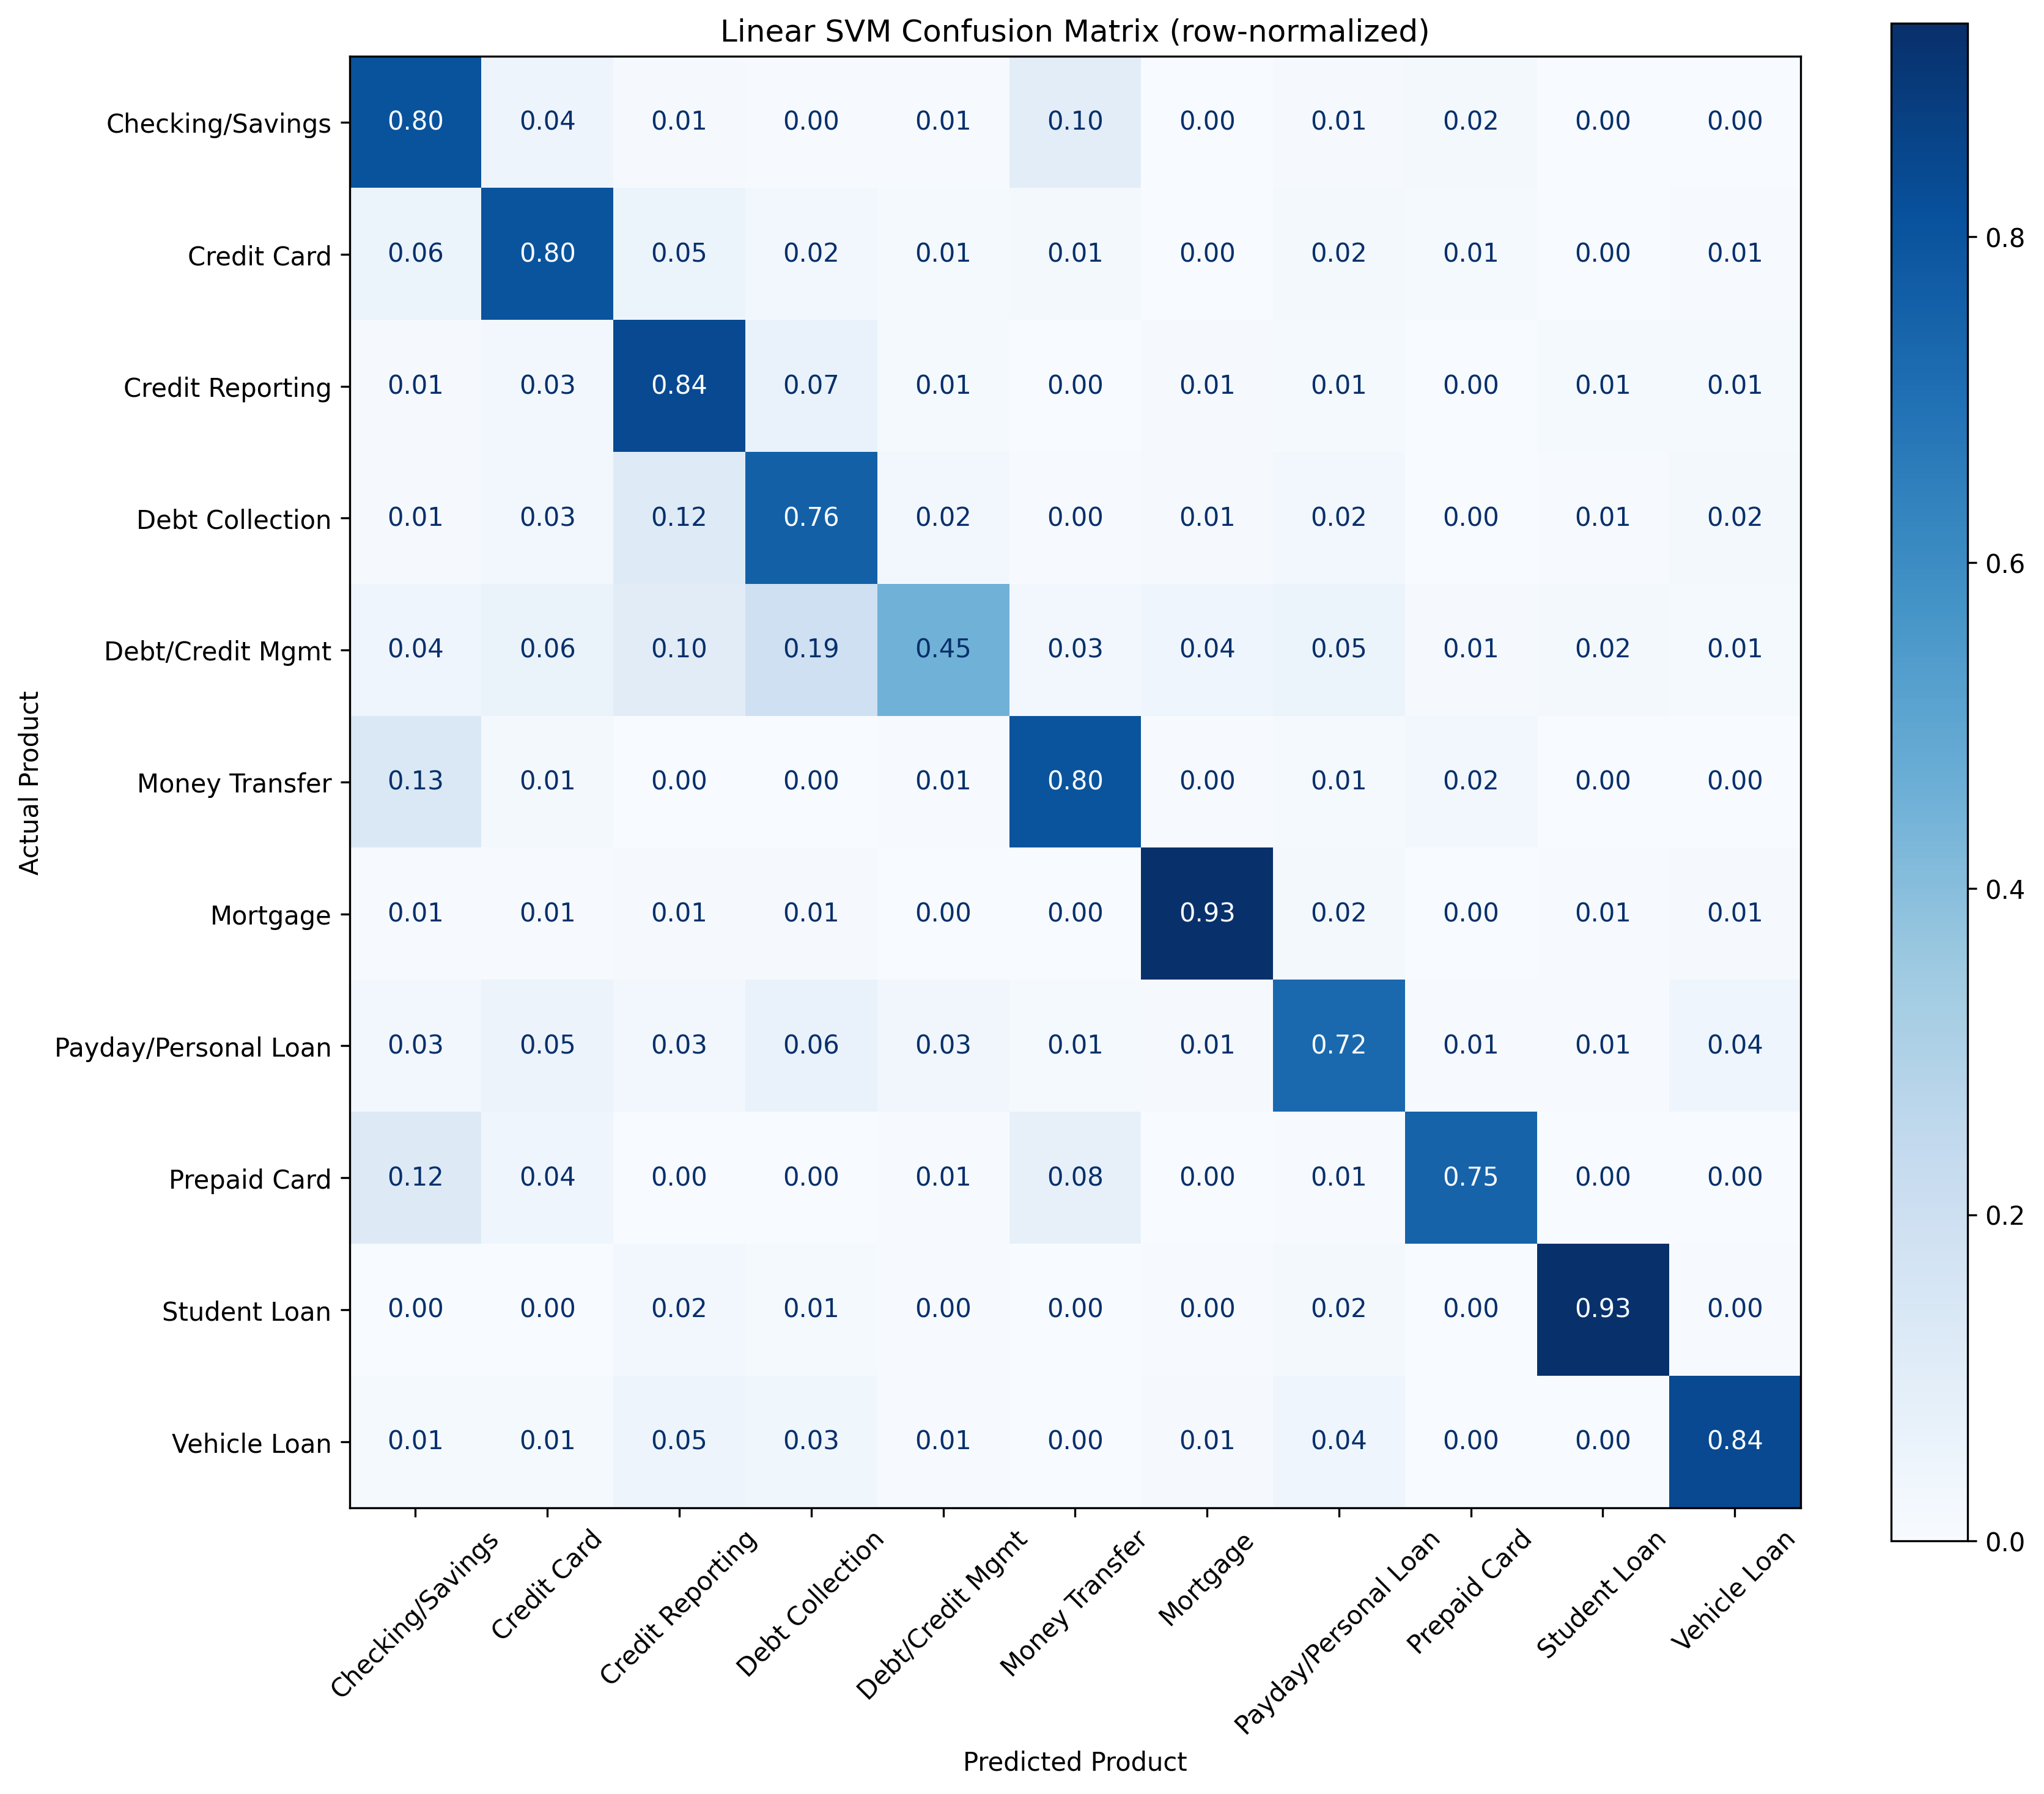
\includegraphics[width=\columnwidth]{figures/linear_svm_confusion_matrix.png}
\caption{Linear SVM confusion matrix on the test set, normalized by row (actual product).}
\label{fig:cm}
\end{figure}

\subsection{Training Behavior}
Naive Bayes and the linear models have no epochs, but the MLP does (Fig.~\ref{fig:loss}). Its training loss falls steadily from 0.87 to 0.33 over 15 epochs, while validation accuracy peaks at 0.782 after epoch 4 and then declines to 0.754. The network starts to memorize the training set after a few passes. Early stopping ends training once validation accuracy has not improved for more than 10 epochs and restores the epoch-4 weights. In the mid-term report, a learning curve for naive Bayes showed a similar ceiling: validation loss flattened at about 40,000 training complaints, so better features and models, not more data, were the way forward.

\begin{figure}[!t]
\centering
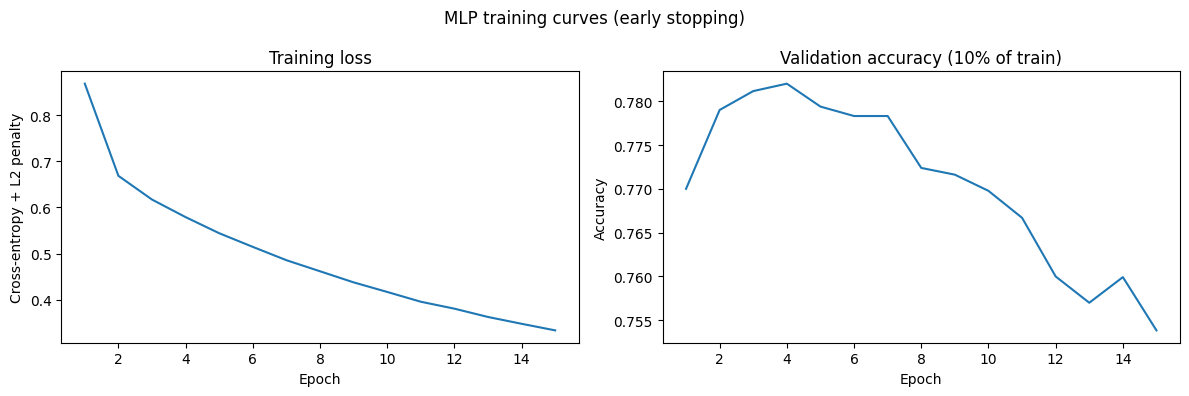
\includegraphics[width=\columnwidth]{figures/mlp_loss_curve.png}
\caption{MLP training loss (left) and validation accuracy on a 10\% hold-out of the training set (right). Early stopping keeps the weights from epoch 4.}
\label{fig:loss}
\end{figure}

\subsection{How Much Does Truncated SVD Keep?}
\label{sec:svd}
Fig.~\ref{fig:svd} shows a linear SVM trained on the first $k$ SVD components. Two components give a macro-F1 of only 0.103, and the curve rises quickly up to about 100 components (0.689, 88\% of the full-TF-IDF score of 0.782). After that it grows slowly: 300 components keep 94\% and 500 keep 96\% (0.749). The components explain little of the variance (12.5\% with 100 components, 24.2\% with 500), because most of the variance is rare, complaint-specific vocabulary. Still, the leftover signal matters for classification, which is why the SVD-300 models in Table~\ref{tab:results} fall short.

\begin{figure}[!t]
\centering
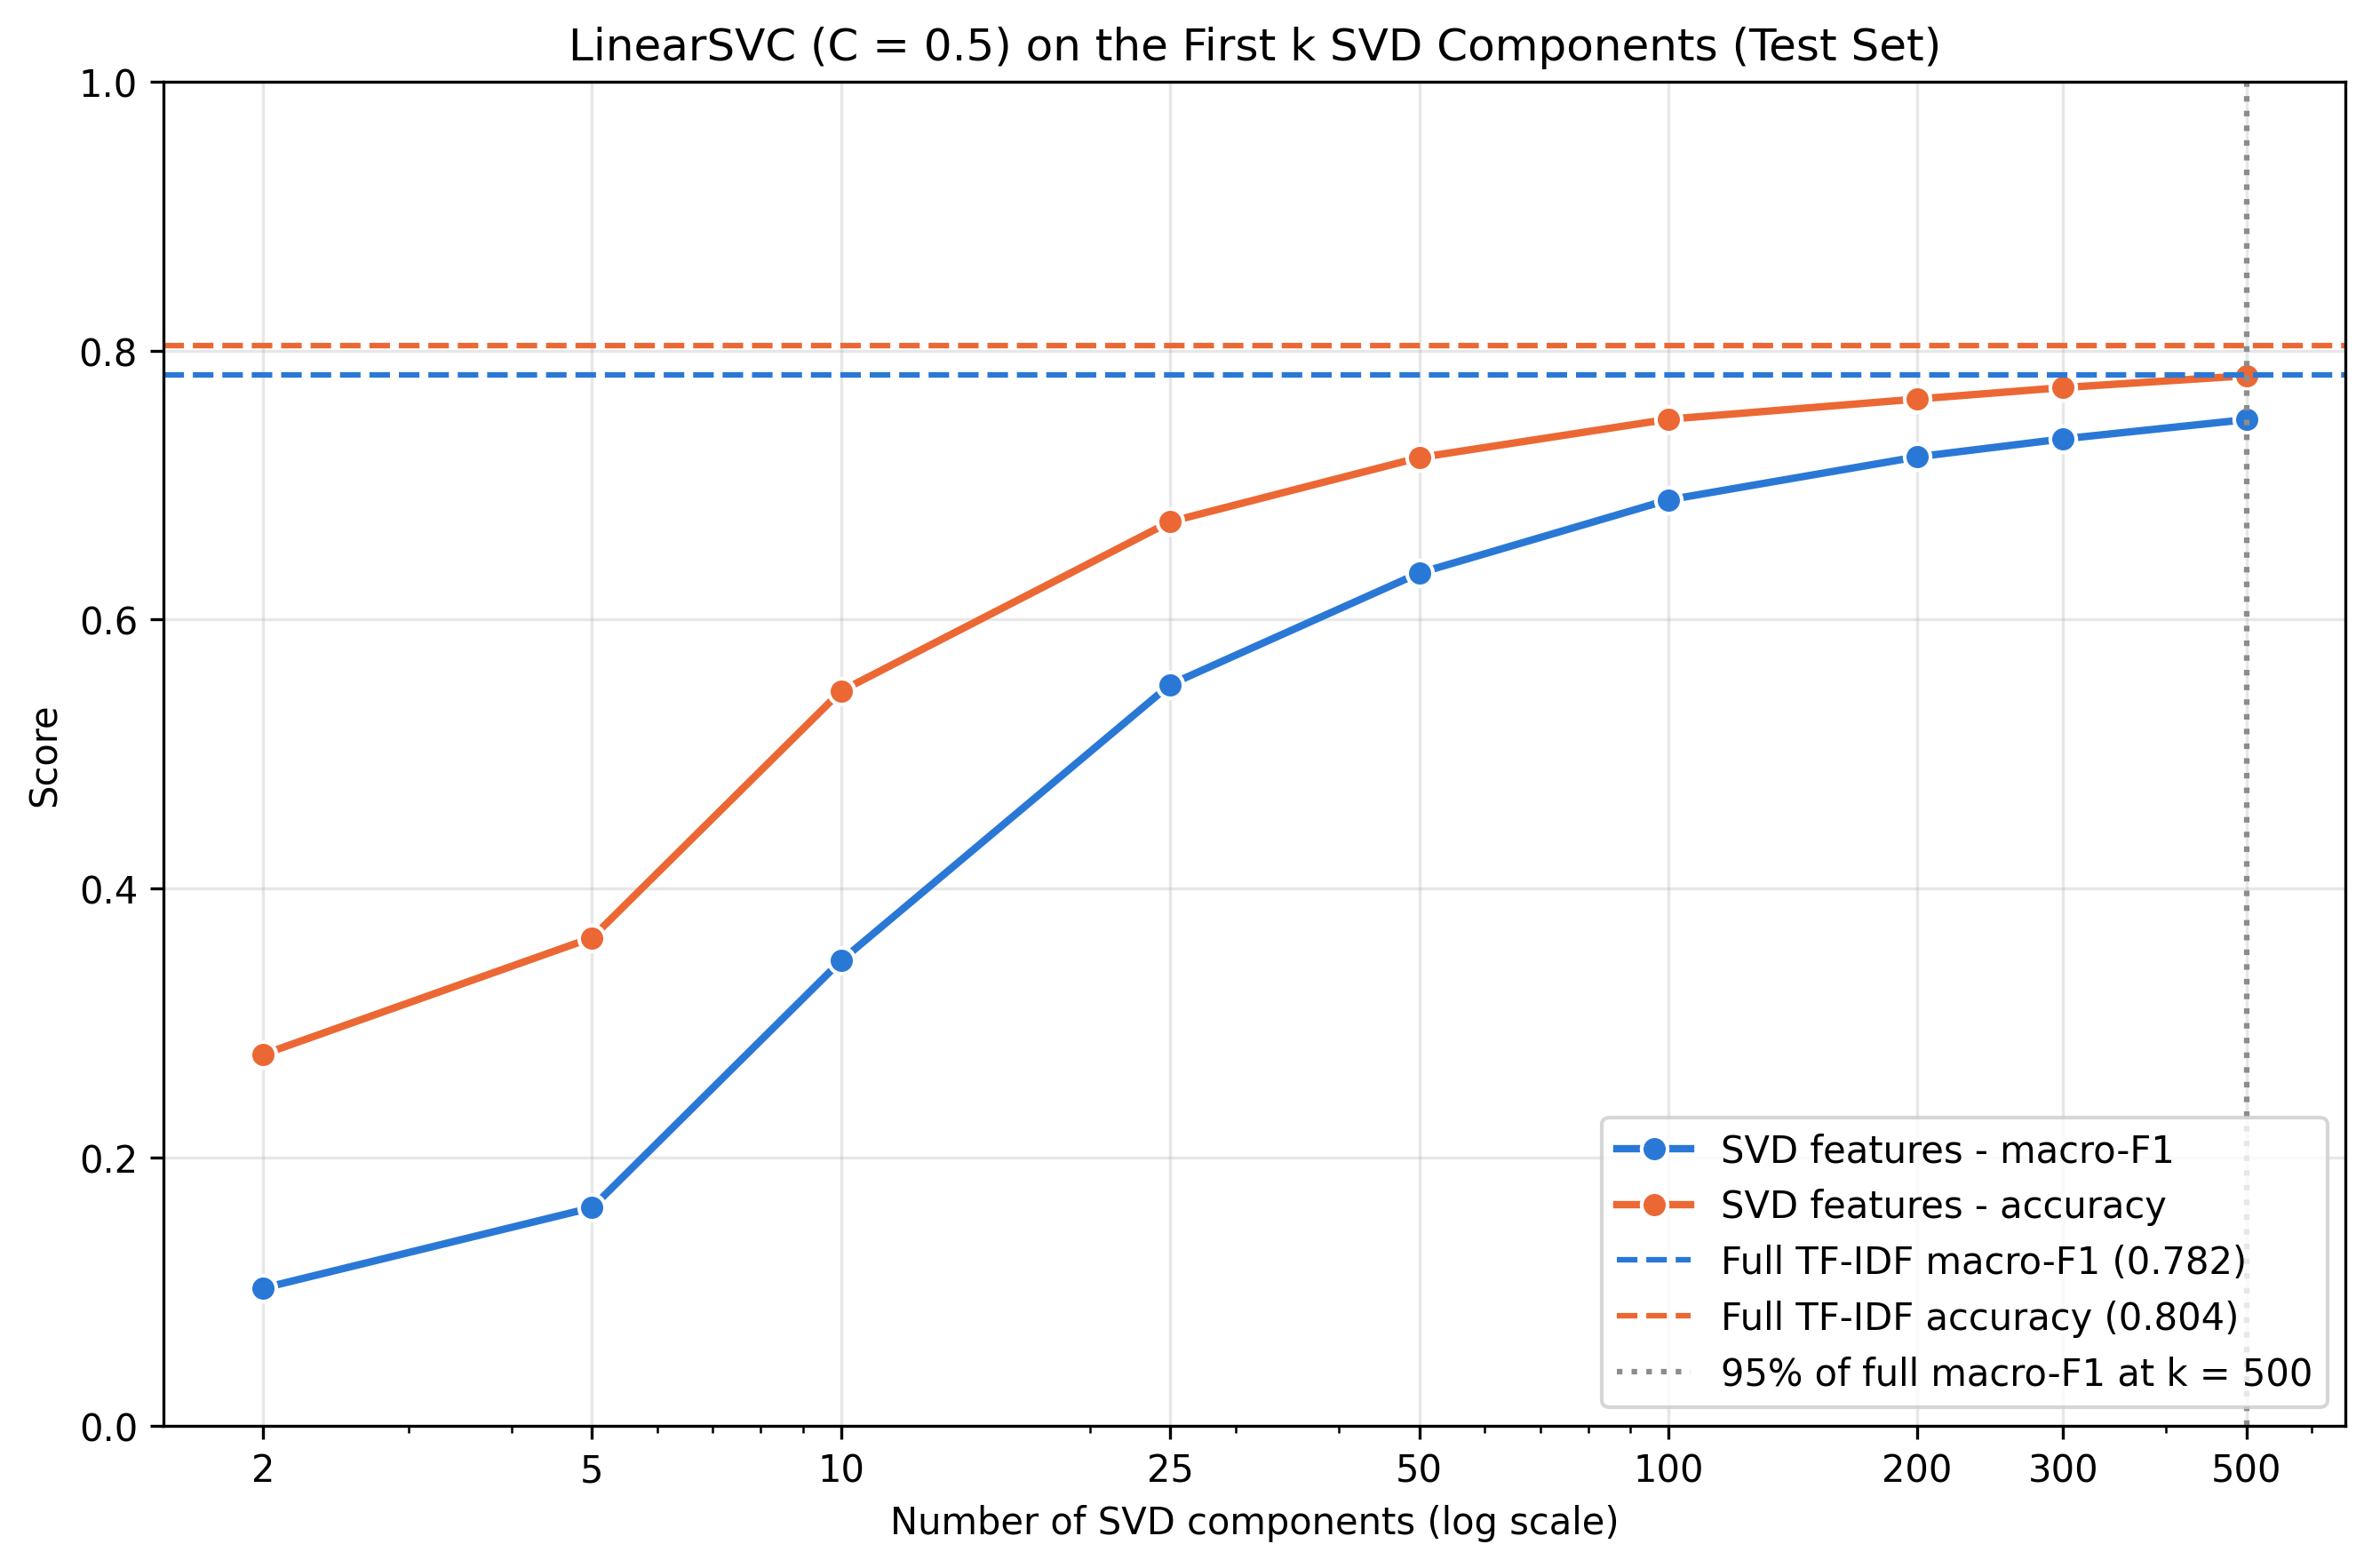
\includegraphics[width=0.95\columnwidth]{figures/svd_components_vs_macro_f1.png}
\caption{Test macro-F1 and accuracy of a linear SVM on the first $k$ SVD components (log scale), compared with the same model on the full 100,000-feature TF-IDF matrix.}
\label{fig:svd}
\end{figure}

\subsection{Complaint Themes}
In a t-SNE map of 10,000 training complaints, student loans, mortgages and vehicle loans form separate islands. Credit reporting overlaps debt collection, and checking/savings overlaps credit cards, money transfer and prepaid cards, the same pairs the classifiers confuse. K-means clusters overlap heavily: the silhouette score stays below 0.1 for every $k$ we tried and peaks at 0.094 for $k=25$. Agreement with the products is low (ARI 0.186, NMI 0.358), because the clusters follow issues and writing styles as well as products. About half are product clusters (93\% student loans, 92\% mortgages). Others are issue clusters that mix products, such as unauthorized transactions and merchant disputes. Several are template campaigns, such as a January 2025 Cash App letter, Zelle letters and credit-repair dispute templates. One cluster is a single company, Wells Fargo. Monetary relief follows the themes: 32.6\% of gift-card complaints get relief, 20.2\% of merchant disputes and 19.3\% of unauthorized-transaction complaints, against 0.5\% or less for every credit-reporting, debt-collection and template cluster.

\subsection{Monetary Relief}
Table~\ref{tab:relief} and Fig.~\ref{fig:pr} show the relief results. With 5.6\% positives, a model with no skill has a PR-AUC of 0.056. Product alone already ranks complaints far better than chance (PR-AUC 0.160, ROC-AUC 0.819), but the narrative more than doubles that (0.357). Adding the product to the text barely helps, because the text already reveals the product. Company adds the most (+0.028), because company policy drives outcomes: the three credit bureaus handle about 26,000 training complaints and almost never pay (Equifax 0.00\%, TransUnion 0.01\%, Experian 0.13\%), while American Express pays in 34.6\% of its complaints. The best model, logistic regression on text, product and company, reaches PR-AUC 0.393 (7.0 times the base rate) and ROC-AUC 0.915. At the threshold chosen on the training folds, it flags 9.8\% of complaints and catches 59\% of the relief cases with 34\% precision. Template letters are not a source of label noise: only 0.2\% of them end in monetary relief. Wang et al.~\cite{wang} report ROC-AUC 0.78 on a temporal split of a different sample, so the two numbers should not be compared directly. A temporal evaluation of our model is future work.

\begin{table}[!t]
\caption{Monetary Relief on the Test Set (32,102 Complaints, 5.6\% Positive)}
\label{tab:relief}
\centering
\footnotesize
\setlength{\tabcolsep}{3.5pt}
\begin{tabular}{@{}lcccc@{}}
\toprule
Model and features & ROC-AUC & PR-AUC & Recall & F1 \\
\midrule
Prevalence baseline & 0.500 & 0.056 & 1.000 & 0.107 \\
LogReg, product only & 0.819 & 0.160 & 0.490 & 0.261 \\
LogReg, text & 0.902 & 0.357 & 0.513 & 0.409 \\
LogReg, text + product & 0.904 & 0.365 & 0.524 & 0.416 \\
\textbf{LogReg, text + product + company} & \textbf{0.915} & \textbf{0.393} & \textbf{0.591} & 0.433 \\
Linear SVM, same features & 0.914 & 0.387 & 0.555 & \textbf{0.434} \\
\bottomrule
\end{tabular}
\end{table}

\begin{figure}[!t]
\centering
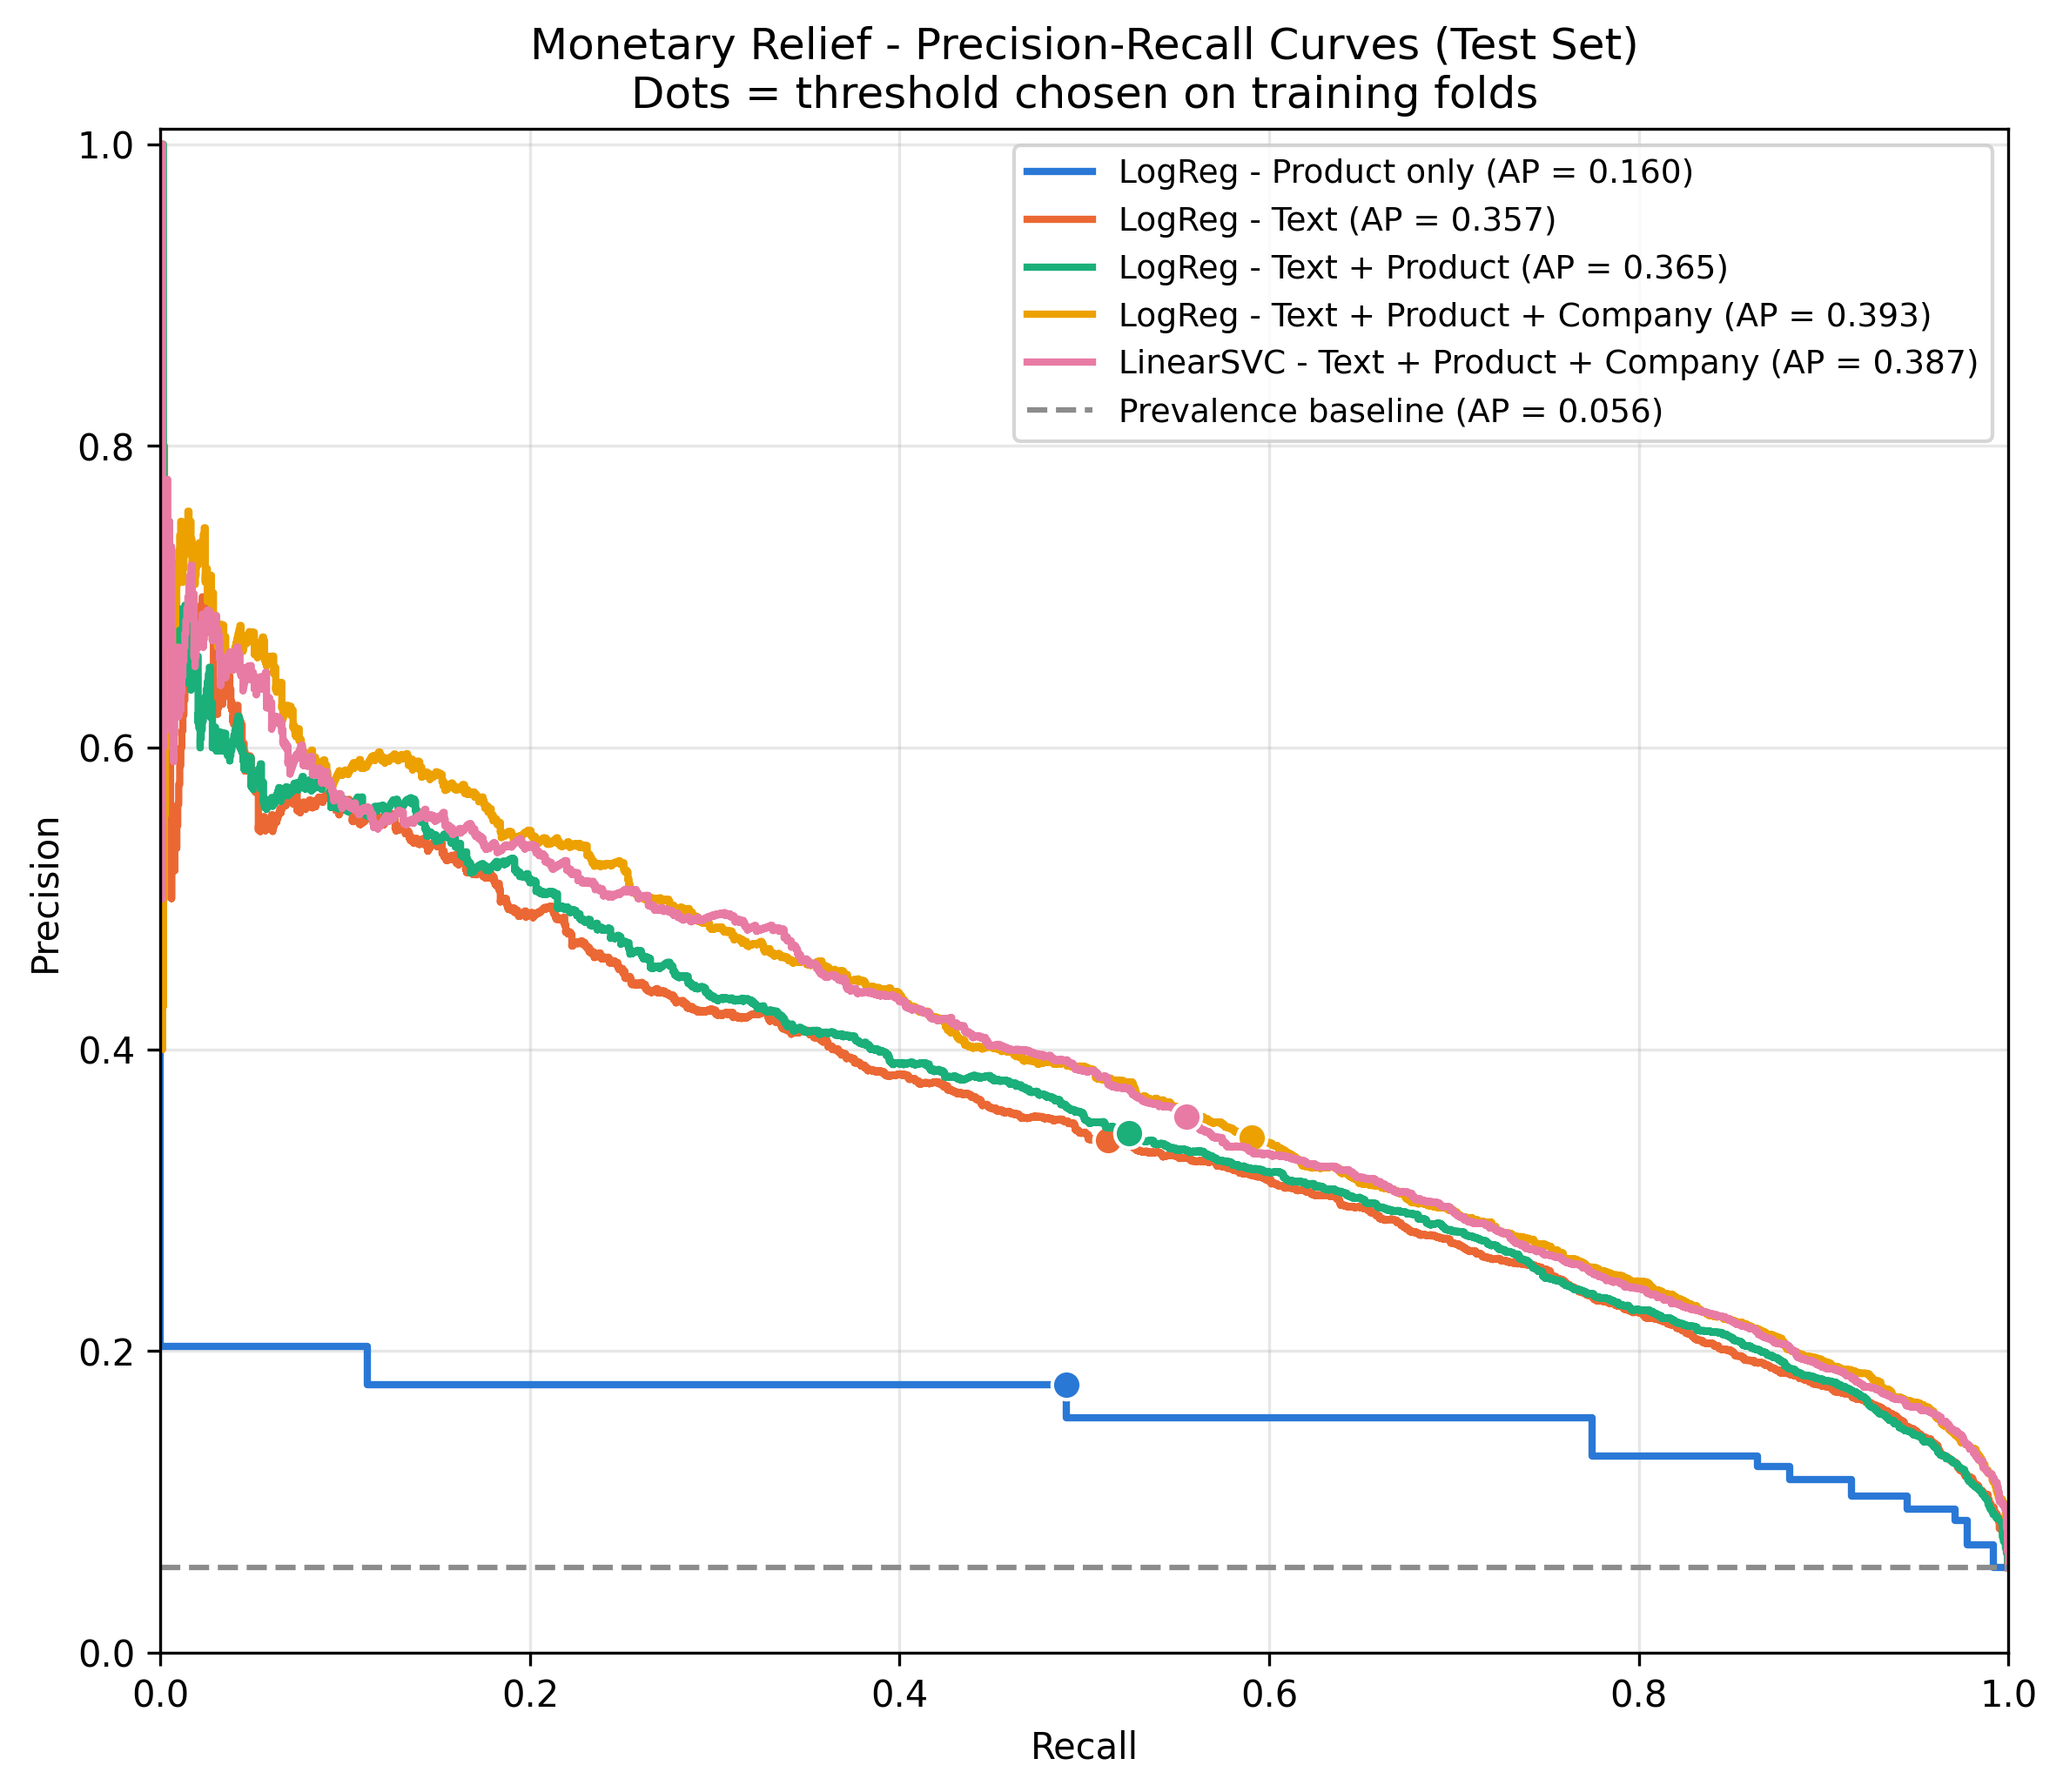
\includegraphics[width=0.9\columnwidth]{figures/relief_pr_curves.png}
\caption{Precision--recall curves for monetary relief. Dots mark the threshold chosen on the training folds.}
\label{fig:pr}
\end{figure}

\subsection{Explanations and Error Analysis}
We analyzed the logistic regression model, which is the model in our demo because it gives probabilities.

\textit{What the model learned.} The terms with the largest weights are often company names, not descriptions of the problem: Equifax, Experian and TransUnion for credit reporting; MOHELA, Nelnet and Aidvantage for student loans; Zelle, PayPal and Cash App for money transfer; and Capital One, Synchrony and Citi for credit cards. Explanations of single predictions show the same thing. A Capital One dispute filed under checking/savings was predicted as a credit card complaint (probability 0.85) mainly because of the words \textit{capital}, \textit{card} and \textit{merchant}.

\textit{Label ambiguity.} The ten most confused product pairs account for half of all errors, and many errors look like ambiguous labels rather than model mistakes, since consumers choose the product themselves. For example, money-transfer complaints about check cashing (77\% error) and money orders (67\% error) describe the same bank-side events as checking-account complaints.

\textit{Confidence.} The model's confidence is informative (Fig.~\ref{fig:conf}). Correct predictions have a median confidence of 0.92 and incorrect ones 0.59. The 46\% of predictions with confidence above 0.9 are 94.9\% accurate, while the 13\% at or below 0.5 are only 43.8\% accurate. If complaints with confidence of 0.7 or less went to a human reviewer, the reviewer would see 29\% of the complaints and catch about 65\% of the errors. Short narratives are harder: complaints under 50 words have a 31.6\% error rate, against 16--18\% for 100 words or more.

\begin{figure}[!t]
\centering
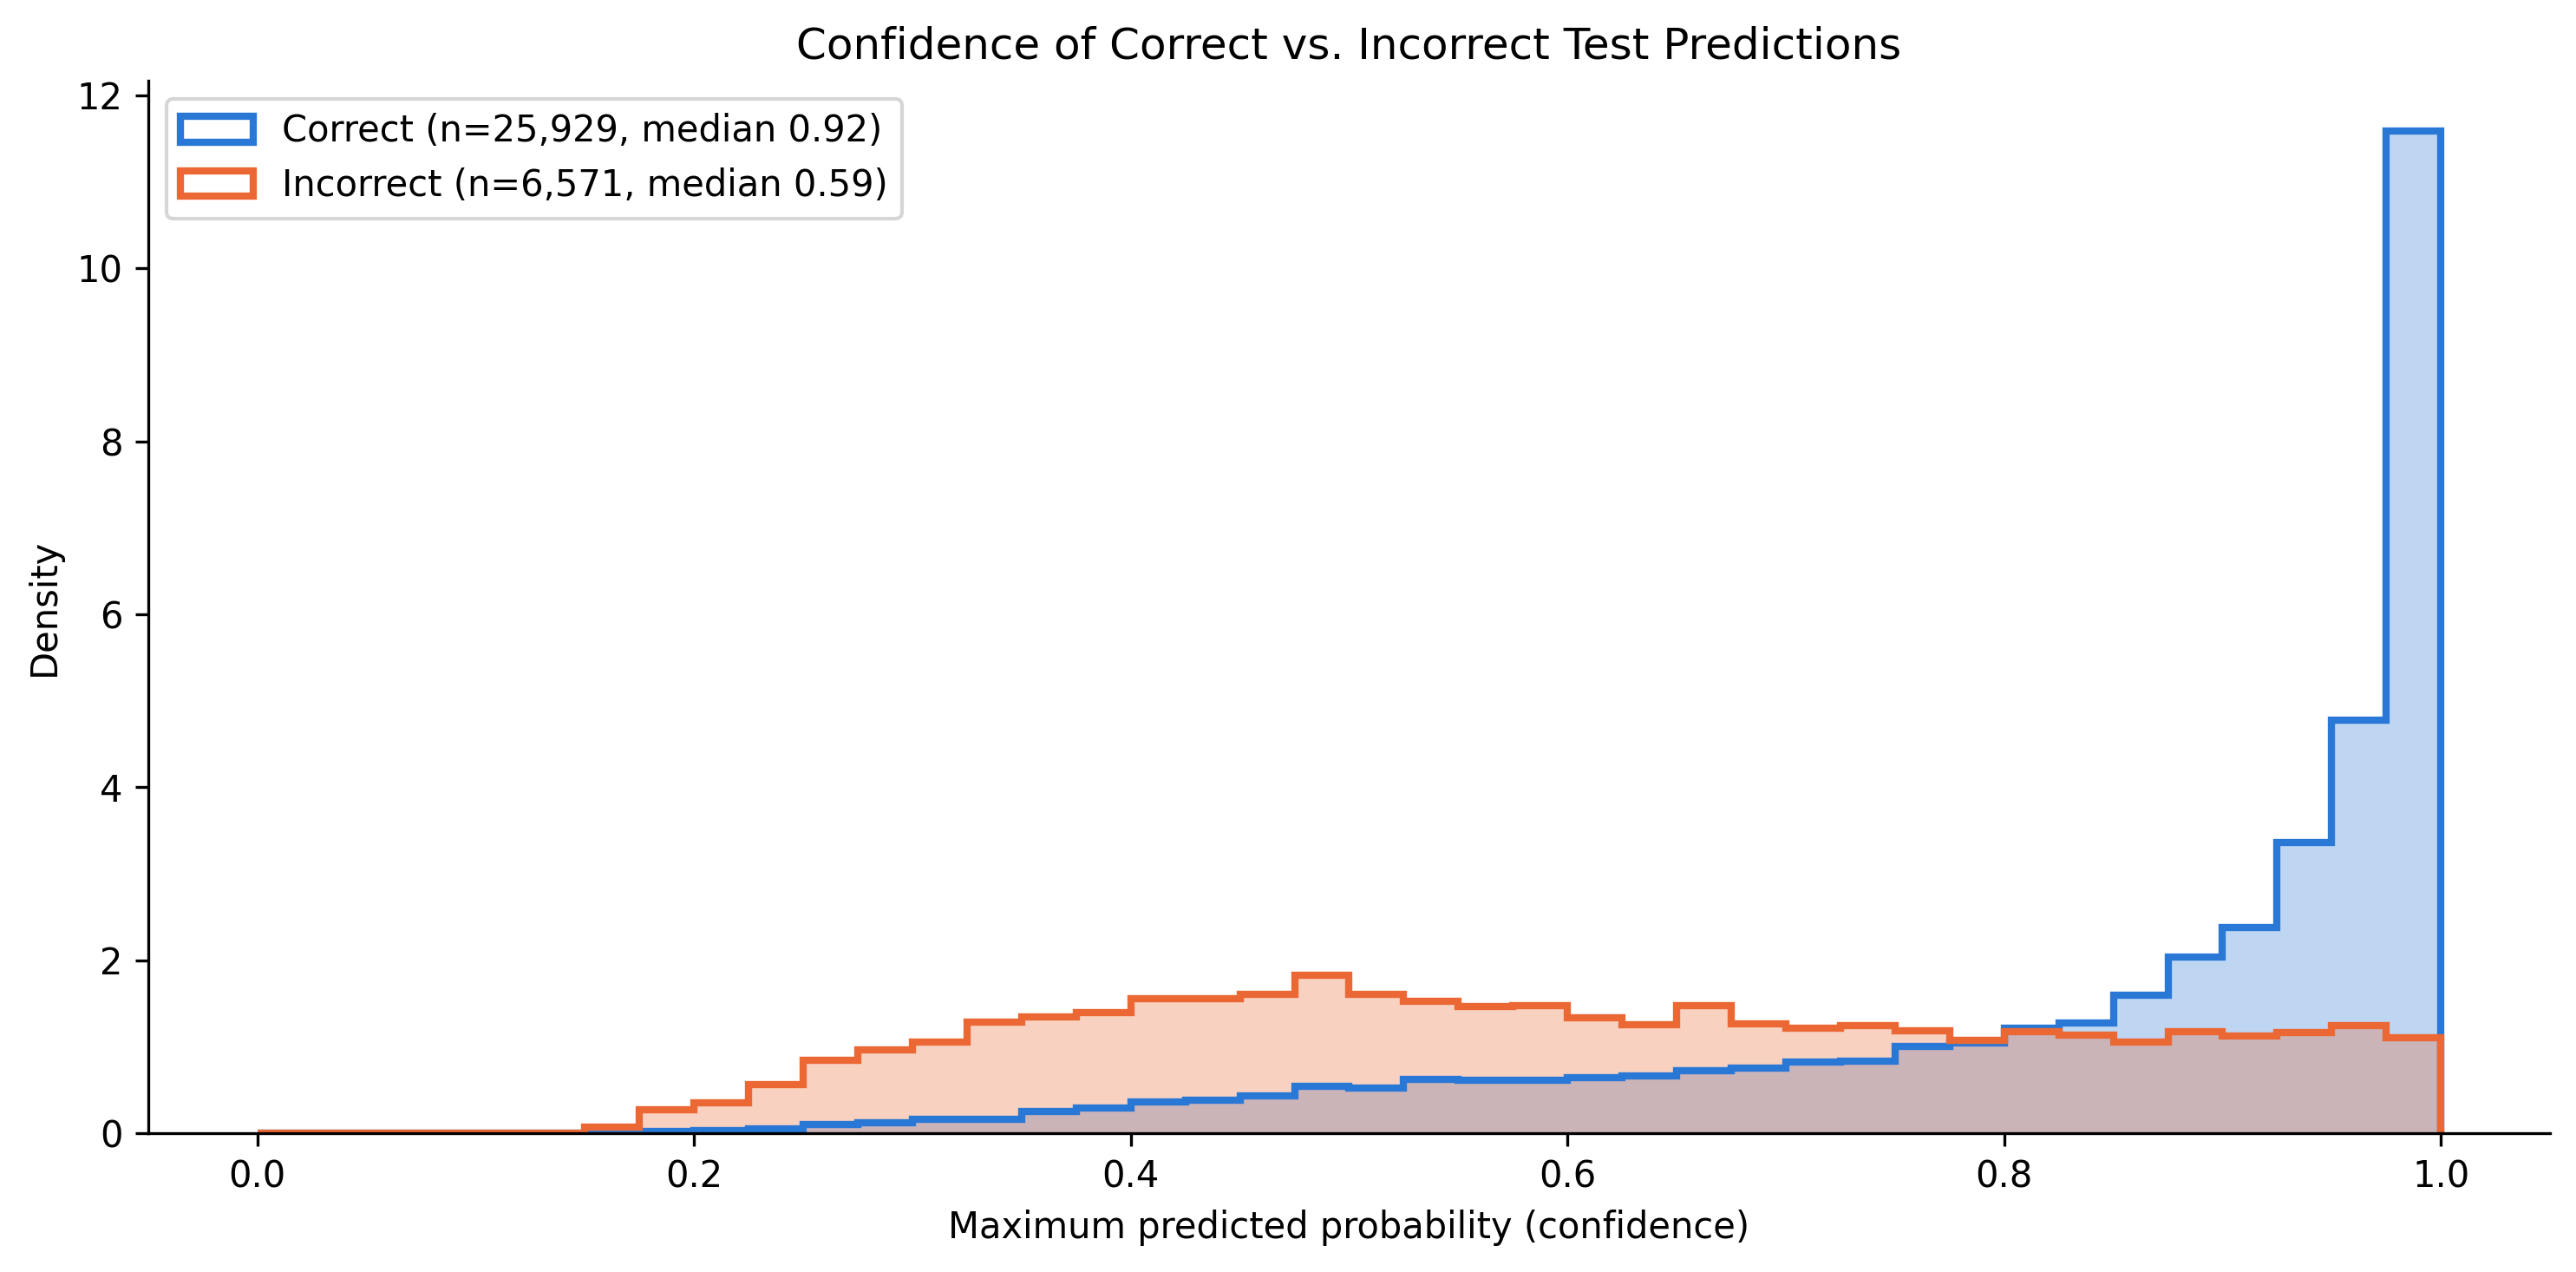
\includegraphics[width=\columnwidth]{figures/error_confidence_distribution.png}
\caption{Confidence (highest predicted probability) of correct and incorrect logistic regression predictions on the test set.}
\label{fig:conf}
\end{figure}

\textit{Leakage check.} Exact duplicates were removed, but lightly edited template letters could still appear in both the training and test sets. We found that 1,818 test complaints (5.6\%) start with the same 200 characters as a training complaint, mostly credit-reporting and money-transfer templates. Accuracy on these complaints is higher (0.957 vs.\ 0.788), but removing them lowers macro-F1 only from 0.776 to 0.771. Template copies inflate our results only slightly and do not drive the model comparison.

\subsection{Demo}
Our Streamlit app takes a pasted narrative (or one of several sample complaints), cleans it with the same function used in training, and shows the three most likely products with their probabilities, a monetary-relief score with a likely/unlikely flag, and the words that pushed the prediction the most. There is no live data feed, because the CFPB no longer publishes new narratives.

\section{Discussion and Limitations}
The main lesson is that, for this task, a well-tuned linear model on sparse word and bigram features beats more complex models trained on compressed features. The remaining errors cluster in a few product pairs whose complaints really do overlap. Some limits apply to our results. First, the capped sample makes the test set more balanced than real complaint traffic, which is 53\% credit reporting, so overall accuracy on real traffic would differ. Second, we used a random split. Template campaigns come in waves (one Cash App campaign appeared in January 2025), so performance on future complaints may be lower. Third, the model relies on company names, which works for known companies but may not transfer to new ones. Fourth, the relief model's probabilities are inflated by class weighting and should be read as a ranking score, not a calibrated probability. Finally, we did not reach our stretch goal of fine-tuning DistilBERT~\cite{distilbert}, because it needs a GPU.

\section{Future Work}
We see five next steps: (1)~fine-tune a transformer such as DistilBERT and compare it with few-shot LLM prompting~\cite{pradhan}; (2)~evaluate on a temporal split to measure drift as new templates and companies appear; (3)~predict the sub-product and issue as well as the product, with a hierarchical classifier; (4)~train with company names masked to test how much the model depends on them; and (5)~calibrate both models and pick review thresholds by cost, so low-confidence complaints go to a human.

\section{Conclusion}
Griev.AI.ance routes CFPB complaints to the right product with 0.784 macro-F1 and 80.6\% accuracy using a linear SVM on TF-IDF features, a 0.089 gain over our naive Bayes baseline, and it ranks monetary-relief complaints at seven times the base rate. Truncated SVD and the nonlinear models did not beat the sparse linear models, but the analysis explained why and showed that confidence scores can send uncertain complaints to people. The whole pipeline, from the archived data to the demo, is reproducible from our notebooks.

\begin{thebibliography}{00}
\bibitem{cfpb} Consumer Financial Protection Bureau, ``Consumer Complaint Database.'' [Online]. Available: \url{https://www.consumerfinance.gov/data-research/consumer-complaints/}
\bibitem{joachims} T. Joachims, ``Text categorization with support vector machines: Learning with many relevant features,'' in \textit{Proc. ECML}, 1998, pp. 137--142.
\bibitem{mccallum} A. McCallum and K. Nigam, ``A comparison of event models for naive Bayes text classification,'' in \textit{AAAI-98 Workshop on Learning for Text Categorization}, 1998.
\bibitem{rennie} J. D. M. Rennie, L. Shih, J. Teevan, and D. R. Karger, ``Tackling the poor assumptions of naive Bayes text classifiers,'' in \textit{Proc. ICML}, 2003, pp. 616--623.
\bibitem{lsa} S. Deerwester, S. T. Dumais, G. W. Furnas, T. K. Landauer, and R. Harshman, ``Indexing by latent semantic analysis,'' \textit{J. Amer. Soc. Inf. Sci.}, vol. 41, no. 6, pp. 391--407, 1990.
\bibitem{bastani} K. Bastani, H. Namavari, and J. Shaffer, ``Latent Dirichlet allocation (LDA) for topic modeling of the CFPB consumer complaints,'' \textit{Expert Syst. Appl.}, vol. 127, pp. 256--271, 2019.
\bibitem{pradhan} M. Pradhan, N. Vemprala, and N. Gudigantala, ``Beyond zero-shot: Enhancing LLM financial complaint classification with relevancy-driven RAG-based few-shot prompting,'' in \textit{Proc. Hawaii Int. Conf. Syst. Sci. (HICSS)}, 2026.
\bibitem{wang} Z. Wang, S. Zhu, and X. Chen, ``From complaint narratives to monetary relief: A hybrid machine learning framework for CFPB consumer complaints,'' arXiv:2606.22664, 2026.
\bibitem{tsne} L. van der Maaten and G. Hinton, ``Visualizing data using t-SNE,'' \textit{J. Mach. Learn. Res.}, vol. 9, pp. 2579--2605, 2008.
\bibitem{distilbert} V. Sanh, L. Debut, J. Chaumond, and T. Wolf, ``DistilBERT, a distilled version of BERT: Smaller, faster, cheaper and lighter,'' arXiv:1910.01108, 2019.
\bibitem{sklearn} F. Pedregosa \textit{et al.}, ``Scikit-learn: Machine learning in Python,'' \textit{J. Mach. Learn. Res.}, vol. 12, pp. 2825--2830, 2011.
\end{thebibliography}

\end{document}
